\subsection{Mesh generation}
\label{subsec:mesh_generation}

The next step in the CFD simulation is to generate the mesh for the computational domain.

Given that our focus is strictly related to the rocket itself and not the flow field around it, we opted for a relatively coarse mesh at the boundary of the domain, and a progressively finer mesh around the rocket.
Having the possibility to do so, we also opted for an unstructured mesh, which allows for a more accurate representation of the geometry at the cost of a higher computational time (manageable in our case given the relatively small size of the domain).

The mesh was generated using \texttt{Mechanical} module.
Default parameters were used for the mesh generation, except of the \textit{Inflaction Layer Mesh} around the rocket.

In Table \ref{tab:mesh_inflaction} we report the parameters that were changed from the default values for the mesh generation around the rocket.

\begin{table}[H]
    \centering
    \begin{tabular}{|r|c|}
        \hline
        \textbf{Parameter}      & \textbf{Value}        \\
        \hline
        Use Automatic Inflation & Program Controlled    \\
        Inflation Option        & First Layer Thickness \\
        First Layer Height      & $1.5^{-3}m$           \\
        Maximum Layers          & $20$                  \\
        Growth Rate             & $1.2$                 \\
        Inflation Algorithm     & Pre                   \\
        View Advanced Options   & No                    \\
        \hline
    \end{tabular}
    \caption{Mesh \textit{Inflation} parameters used.}
    \label{tab:mesh_inflaction}
\end{table}

In Table \ref{tab:mesh_statistics} we report the statistics of the generated mesh.

\begin{table}[H]
    \centering
    \begin{tabular}{|c|c|}
        \hline
        \textbf{Parameter} & \textbf{Value} \\
        \hline
        Number of Nodes    & $73473$        \\
        Number of Elements & $177218$       \\
        \hline
    \end{tabular}
    \caption{Mesh statistics.}
    \label{tab:mesh_statistics}
\end{table}

\begin{figure}[H]
    \centering
    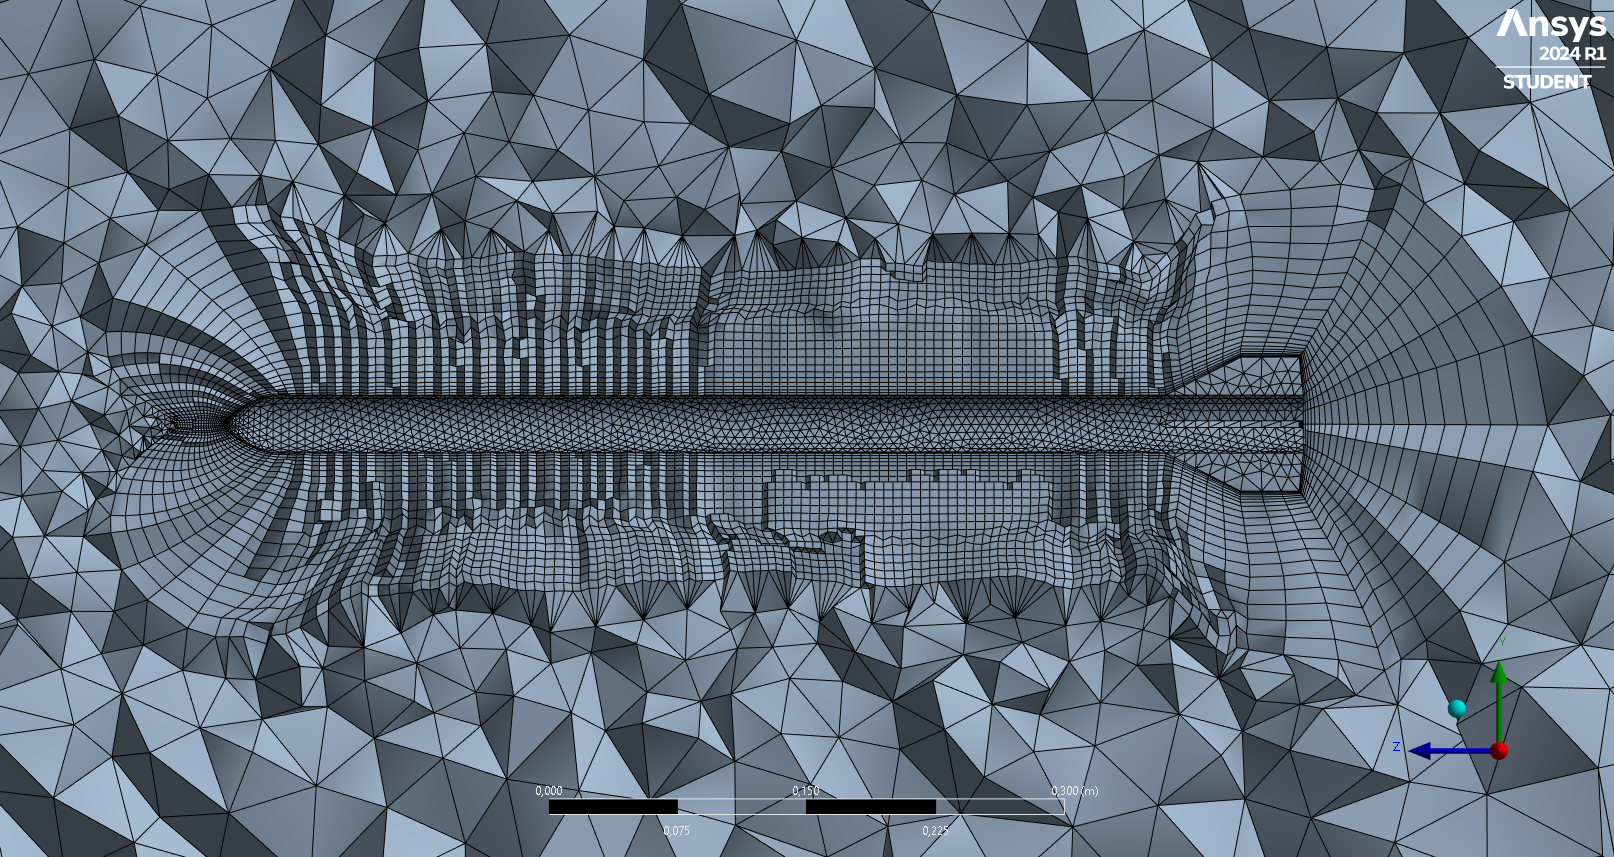
\includegraphics[width=.7\textwidth]{img/PreRunning/Mesh_sectioned.png}
    \caption{The inflation layer mesh around the rocket body is clearly visible.}
    \label{fig:mesh_sectioned}
\end{figure}

\begin{figure}[H]
    \centering
    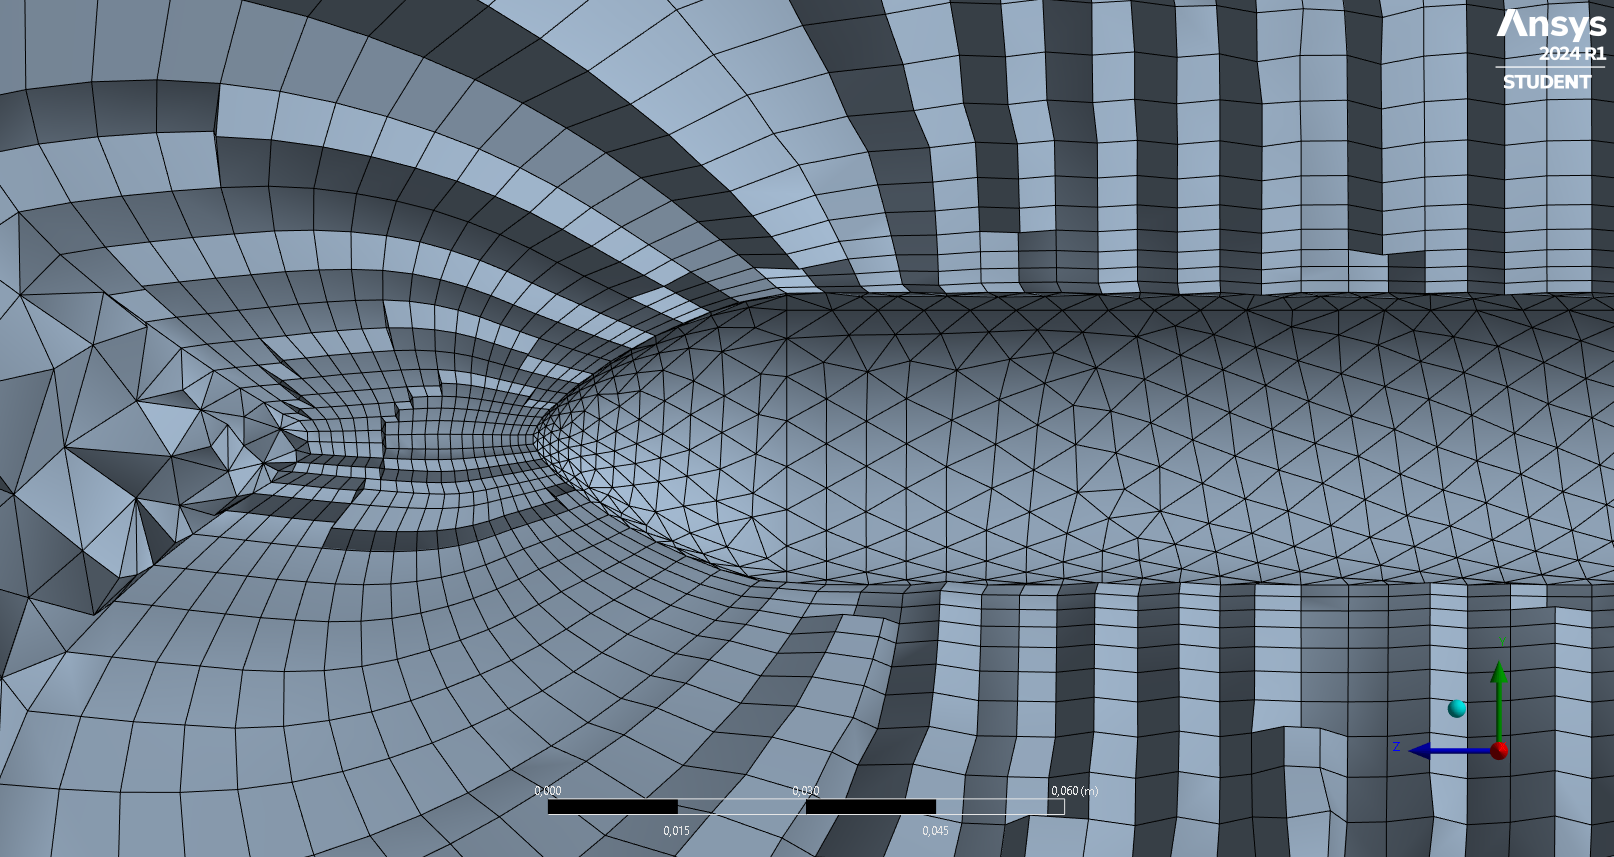
\includegraphics[width=.7\textwidth]{img/PreRunning/Mesh_sectioned_nose.png}
    \caption{Mesh details around the rocket nose cone. Due to the relatively high curvature of the nose cone, the generated mesh is finer with respect to the linear element of the rocket body.}
    \label{fig:mesh_sectioned_nose}
\end{figure}